\documentclass{article}


% if you need to pass options to natbib, use, e.g.:
\PassOptionsToPackage{numbers, compress}{natbib}
%\PassOptionsToPackage{compress}{natbib}
% before loading neurips_2023


% ready for submission
%\usepackage[final]{neurips_2023}


% to compile a preprint version, e.g., for submission to arXiv, add add the
%[preprint] option:
\usepackage[preprint]{neurips_2023}


% to compile a camera-ready version, add the [final] option, e.g.:
%     \usepackage[final]{neurips_2023}


% to avoid loading the natbib package, add option nonatbib:
%     \usepackage[nonatbib]{neurips_2023}


\usepackage[utf8]{inputenc} % allow utf-8 input
\usepackage[T1]{fontenc}    % use 8-bit T1 fonts
\usepackage{hyperref}       % hyperlinks
\usepackage{url}            % simple URL typesetting
\usepackage{booktabs}       % professional-quality tables
\usepackage{amsfonts}       % blackboard math symbols
\usepackage{nicefrac}       % compact symbols for 1/2, etc.
\usepackage{microtype}      % microtypography
\usepackage{xcolor}         % colors

% Added by Jacob
\usepackage[colorinlistoftodos,color=yellow]{todonotes}
\usepackage{subfiles} % Best loaded last in the preamble
%\usepackage{authblk}
%\author[1]{Alison Carefully}
%\usepackage{emoji}

%%% Supplementary Figure labeling. Not standard neurips formatting - 
\newcommand{\beginsupplement}{%
        \setcounter{table}{0}
        \renewcommand{\thetable}{S\arabic{table}}%
        \setcounter{figure}{0}
        \renewcommand{\thefigure}{S\arabic{figure}}%
        \renewcommand{\theHfigure}{Supplement.\thefigure}
     }

% Recommended, but optional, packages for figures and better typesetting:
\usepackage{microtype}
\usepackage{graphicx}
\usepackage{subfigure}
\usepackage{booktabs} % for professional tables




% \title{MosaicBERT: An Efficient Architecture for Accelerated BERT Pretraining - Draft for ICML Workshop}
% \title{MosaicBERT: Pretraining BERT from Scratch for \$20}
\title{DocumentBERT: A Bidirectional Document Encoder for Knowledge Base Retrieval}



% The \author macro works with any number of authors. There are two commands
% used to separate the names and addresses of multiple authors: \And and \AND.
%
% Using \And between authors leaves it to LaTeX to determine where to break the
% lines. Using \AND forces a line break at that point. So, if LaTeX puts 3 of 4
% authors names on the first line, and the last on the second line, try using
% \AND instead of \And before the third author name.

%\author[1]{Alison Carefully}
%\author[2]{Joe Schmoe}
%\affil[1]{Department of Mathematics, University X}
%\affil[2]{Department of Biology, University Y}

\author{%
  Arijit Das\thanks{Code can be found at \href{https://mosaicbert.github.io}{\url{mosaicbert.github.io}}} \\
  \texttt{Machine Learning Group, ERGO Group AG}\\
  \texttt{arijit.das@selfsupervised.de}\\
}


\begin{document}


\maketitle

\begin{abstract}
    Although BERT-style encoder models are heavily used in NLP research, many researchers need to pre-train their BERTs from scratch due to the high cost of training.
    Since BERT first rose to prominence in the past half-decade, many advances have been made with other transformer architectures and training configurations that have yet to be systematically incorporated into BERT.
    Here, we introduce MosaicBERT, a BERT-style encoder architecture and training recipe empirically optimized for fast pretraining.
    This efficient architecture incorporates FlashAttention, Attention with Linear Biases (ALiBi), Gated Linear Units (GLU), a module to dynamically remove padded tokens, and low-precision LayerNorm into the classic transformer encoder block.
    The training recipe includes a 30\% masking ratio for the Masked Language Modeling (MLM) objective, bfloat16 precision, and vocabulary size optimized for GPU throughput, in addition to best practices from Roberta and other encoder models.
    When trained from scratch on the C4 dataset, this base model achieves a downstream average GLUE (dev) score of 79.6 in 1.13 hours on 8 A100 80 GB GPUs at the cost of roughly \$20.
    We plot extensive accuracy vs. pretraining speed Pareto curves and show that MosaicBERT base and large are consistently Pareto optimal when compared to a competitive BERT base and large.
    This empirical speed-up in pretraining enables researchers and engineers to train custom BERT-style models at low cost instead of fine-tuning existing generic models. 
    We open-source our model weights and code.
\end{abstract}



\section{Introduction}


BERT has been the workhorse of modern natural language processing (NLP) since its introduction in 2018 \citep{devlin2018bert}. 
Even in the era of large language models (LLMs), BERT-style encoder models are still quite relevant; for example, encoder models are used for vector database embeddings and retrieval augmented generation in tandem with LLMs \citep{karpukhin2020dense,lewis2020retrieval,izacard2022unsupervised,wang2022text,shi2023replug}.
In the past half-decade since BERT first rose to prominence, however, many advances have been made with other transformer architectures and training configurations that have yet to be systematically incorporated into BERT \citep{dauphin2017language,press2021train,dao2022flashattention}. In this study we empirically show that these speed optimizations can successfully be incorporated into the classic BERT architecture and training recipe.

BERT-style models are typically trained in two stages: an initial self-supervised pretraining phase that builds general representations of language, and a subsequent supervised finetuning phase that uses those representations to address a specific task.
The pretraining stage for BERT models has historically been computationally expensive; in the original BERT study, for example, the authors trained their models for 4 full days on 16 Google TPUs. 
In recent years, however, the time and cost to train BERT models has dropped significantly. One widely cited paper from 2021 successfully reduced the training time of BERT-Large to 24 hours on 8 Titan V-12 GPUs \citep{izsak2021train}, and another very recent paper trained a competitive BERT-Base model on a single consumer GPU in only 24 hours \citep{geiping2023cramming}. Our work builds on these trends.

In this study, we introduce our optimized MosaicBERT architecture and show that certain architectural choices for BERT-style encoders lead to accuracy vs. time Pareto improvements in pretraining. We do this by empirically comparing MosaicBERT with an optimal BERT baseline that does \textit{not} incorporate our architectural changes but \textit{does} have non-architectural optimizations such as fast data streaming and optimal floating point precision. We then evaluate on the classic GLUE benchmark \citep{wang2018glue}.

It can often be difficult to understand the effects of model architecture modifications and training hyperparameter choices by simply reporting a few numbers in a table, as is traditionally done in ML papers. A few numbers in a table can obscure differences in the training data, objective function, batch size, training duration, learning rate schedule and many other details. Since our main goal in this study is to show how combinations of architecture choices lead to improvements in both \textit{accuracy} and \textit{training time}, we make the choice to plot accuracy vs. training time Pareto curves for all models (for example, in Figure \ref{fig:intro_figure}B). Certain architecture changes might lead to an increase in throughput, but a decrease in accuracy (e.g. changes to the floating point precision); other changes might lead to an increase in accuracy but take a much longer time to converge (e.g. increasing the model size). Accuracy vs. training time Pareto curves enable us to adequately asses all these changes (see Appendix for a more detailed discussion on Pareto curves).



%One widely cited paper from 2021 pinned the price of pretraining BERT-Large to baseline accuracy at \$300-\$400 \citep{izsak2021train}.\todo{in their final version from EMNLP Nov 2021, they changed it to \$50-100} 
%show that high-quality BERT models can be pretrained from scratch surprisingly quickly. 







\begin{figure}
    \centering
    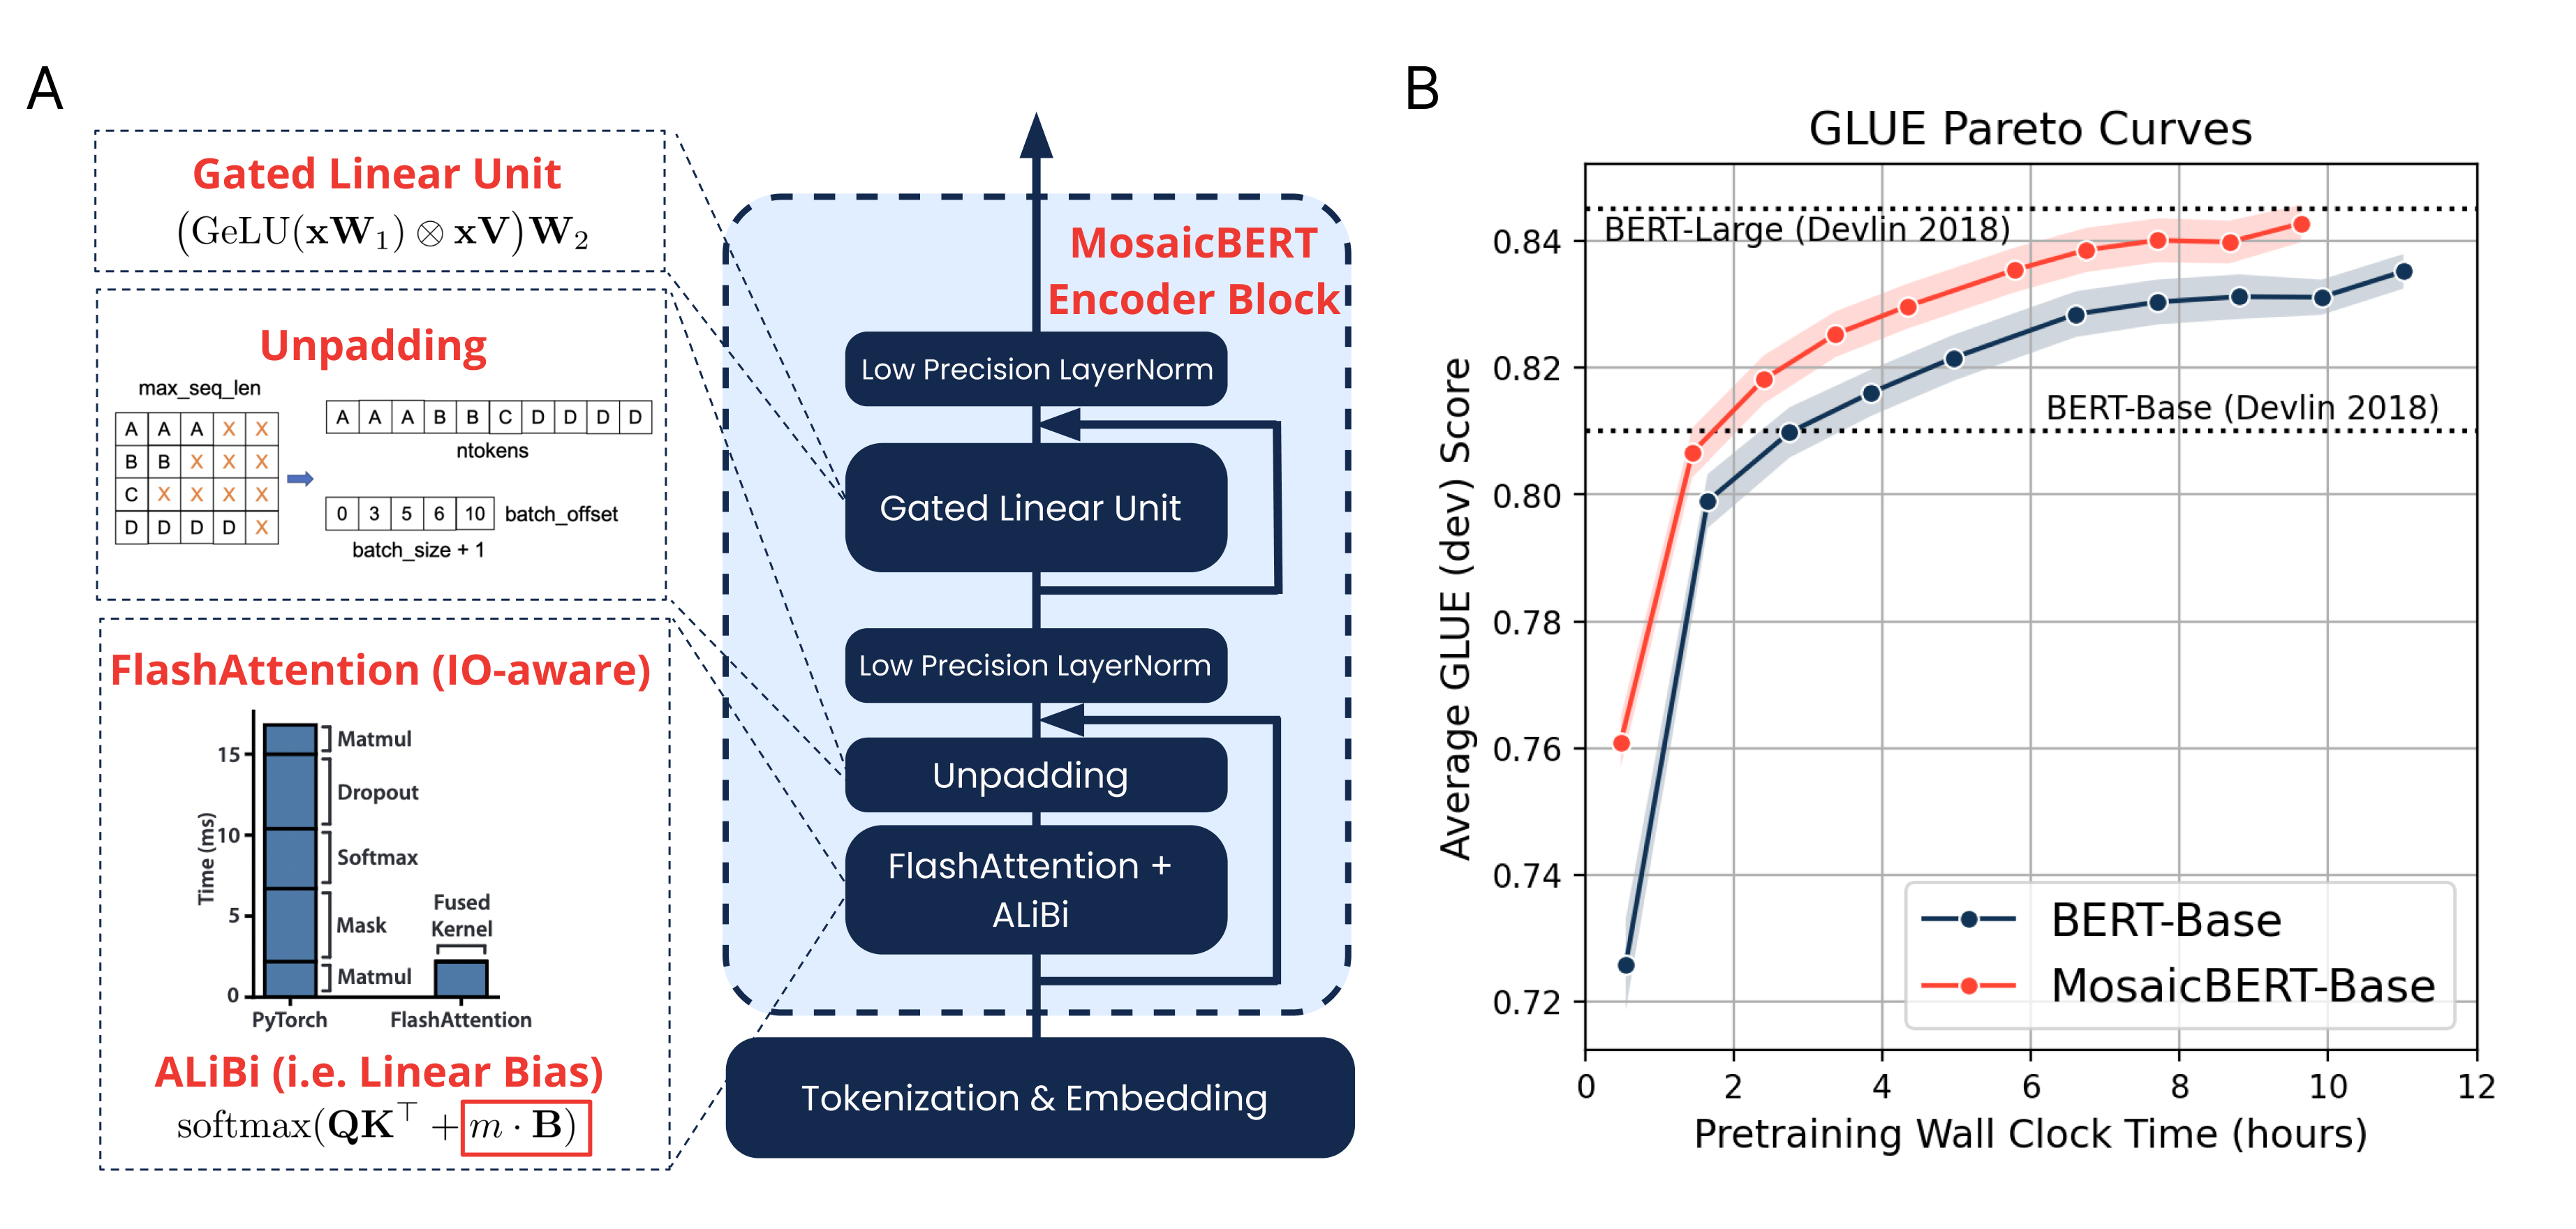
\includegraphics[width=\textwidth]{figures/Figure-1-high-res-12-29-1217am.png}
    \caption{(A) Schematic of MosaicBERT architecture (B) Pareto curves of average GLUE (dev) scores for MosaicBERT-Base and the standard BERT-Base.  Error bars indicate 95\% confidence interval over n=5 pretraining seeds. All training was on $8\times$A100-80GB GPUs. FlashAttention schematic adapted from \cite{dao2022flashattention}, and unpadding schematic adapted from \cite{zeng2022boosting}).}
    \label{fig:intro_figure}
\end{figure}
The contributions of this work are as follows:
\begin{itemize}
    \item We implement a new BERT-style encoder architecture that optimizes pretraining speed and accuracy. This architecture combines FlashAttention \citep{dao2022flashattention}, ALiBi \citep{press2021train}, Gated Linear Units \citep{dauphin2017language,shazeer2020glu}, a dynamic unpadding module \citep{zeng2022boosting}, and low precision LayerNorm.
    \item We show that MosaicBERT base achieves the downstream average GLUE (dev) score of 79.6 in 1.13 hours on $8\times$A100 80 GB GPUs at a cost of roughly \$20 on a standard cloud provider.
    \item We characterize the accuracy vs. pretraining time Pareto frontier for MosaicBERT-Base and Large, and empirically show that the performance of MosaicBERT-Base and Large is Pareto optimal relative to BERT-Base and Large.
    \item We characterize the relative throughput properties of each of MosaicBERT's architecture and design choices via ablations.
    \item  We characterize the tradeoff between model size and training duration, and show that BERT-Large performance only surpasses BERT-Base performance after extensive training. We open-source our model weights and code at \href{https://mosaicbert.github.io}{\url{mosaicbert.github.io}}.
\end{itemize}

Finally, we note that the ideas explored in this study are directly applicable to LLM pretraining, and directly motivated many of the architecture choices around MosaicML's MPT-7B and MPT-30B large language models  \citep{MosaicML2023IntroducingMPT7B,MosaicML2023IntroducingMPT30B}.



\begin{table}[h]
\begin{tabular}{p{4.0cm} p{1.6cm} p{1.0cm} p{2.0cm} p{1.9cm} p{1.cm}}
\toprule

\textbf{Model Architecture} & \textbf{GLUE (dev)} & \textbf{Training (hours)} & \textbf{Hardware} & \textbf{Pretraining Corpus} & \textbf{Params} \\
\midrule

MosaicBERT-Base (ours)  & 79.6 & 1.13  & $8\times$A100-80 & C4 & 137M \\ 

MosaicBERT-Base (ours)  & 82.2 & 2.81  & $8\times$A100-80 & C4 & 137M \\ 

MosaicBERT-Base (ours) & 83.2 & 4.6  & $8\times$A100-80 & C4 & 137M \\ 

MosaicBERT-Base (ours) & 83.4 & 5.27  & $8\times$A100-80 & C4 & 137M \\ 

\midrule

BERT-Base (our benchmark)  & 83.2 & 11.5  & $8\times$A100-80 & C4 & 110M \\ 

\midrule

BERT-Base \citep{devlin2018bert,geiping2023cramming} & 81.0 & 96 & $16\times$TPU & Wiki+BookC & 110M \\ 
BERT-Base \citep{geiping2023cramming} & 73.6 & 24  & 1 RTX A6000 & Wiki+BookC & 110M \\
CrammingBERT-Base \citep{geiping2023cramming} & 80.4 & 24  & 1 RTX A6000 & Wiki+BookC & 110M \\
BERT-Large \citep{devlin2018bert,liu2019roberta} & 84.1 & 96 & $64\times$TPU & Wiki+BookC  & 340M \\ 
\bottomrule
%BERT-Large \citep{izsak2021train} & 78.5 & 24  & $8\times$Titan-V-12 & Wiki+Books & 110M \\ % THIS IS TEST SET
%RoBERTa-Large \citep{izsak2021train} & 83.4 & 24  & $8\times$Titan-V-12 & Wiki+Books & 340M \\ \hline % THIS IS TEST SET
\end{tabular}
\caption{Average GLUE (dev) score across various efficient BERT implementations. Average includes all 8 GLUE tasks. BERT-Base average GLUE scores on the dev set as reported by \cite{geiping2023cramming}, Table 3. BERT-Large average GLUE scores on the dev set as reported by \citep{liu2019roberta}, Table 5. Note that the original training set for BERT was pretrained on 40 epochs of English Wikipedia and BookCorpus \citep{zhu2015aligning}, while MosaicBERT was pretrained on the Colossal Cleaned Common Crawl (C4) corpus \citep{raffel2020exploring}.} %\textbf{TODO: confirm they are all on the dev set}
\label{tab:bert_comparison}
\end{table}

\section{Methods}


In order to build MosaicBERT, we incorporated architectural choices from the recent transformer literature. These include FlashAttention \citep{dao2022flashattention}, ALiBi \citep{press2021train}, training with dynamic unpadding \citep{zeng2022boosting}, low precision LayerNorm, and Gated Linear Units \citep{dauphin2017language,shazeer2020glu} (Figure \ref{fig:intro_figure}). Before describing these modifications in detail, we first review the classic BERT architecture and how we chose a strong baseline.

Since our goal here is to show relative improvements in training time and final accuracy, we do not attempt to beat state of the art models for finetuning benchmarks such as GLUE \citep{wang2018glue}. These SOTA models are often trained for much longer (e.g. \citep{liu2019roberta}) and are larger than the models we explore in this study \citep{clark2020electra,he2021debertav3}.
%\todo{Add more sources here}.

\subsection{Choosing a Strong BERT Baseline}

The basic transformer block used in BERT models consists of (1) the attention mechanism and (2) the feed forward layers. This block is then repeated depending on the model size; BERT-Base has 12 repeated transformer blocks, while BERT-Large has 24. 

For our baseline BERT-Base, we used the exact architecture of BERT from \cite{devlin2018bert};\footnote{The Hugging Face \texttt{bert-base-uncased} model has been downloaded 62 million times, more than any other model on the Hugging Face hub.} this includes a hidden size of 768, an intermediate size of 3072, 12 attention heads and 12 hidden layers, as well as the GeLU activation function, and learned positional embeddings. For our baseline BERT-Large, we used  the exact architecture of BERT-Large from \cite{devlin2018bert}, which has a hidden size of 1024, an intermediate size of 4096, 16 attention heads, and 24 hidden layers.

While MosaicBERT-Base (i.e. 12 hidden layers) and Large (i.e. 24 hidden layers) stay true to this general structure, we introduce modifications that affect both the attention mechanism and the feedforward layers.

%NEED TO CLARIFY ROBERTA SOMEWHERE. These same architecture choices hold for RoBERTa Base and Large






\subsection{MosaicBERT Architecture Modifications for Fast Pretraining}

The MosaicBERT architecture modifies the original BERT architecture in both the attention layers and the feedforward layers.

\subsubsection{Modifications to the Attention Mechanism}
\textbf{FlashAttention}: The recently proposed FlashAttention layer reduces the number of read/write operations between the GPU HBM (high bandwidth memory, i.e. long-term memory) and the GPU SRAM (i.e. short-term memory) \citep{dao2022flashattention} (see also \citep{rabe2021self}). We modified the FlashAttention module built by Hazy Research with OpenAI’s triton library in order to flexibly incorporate ALiBi \citep{tillet2019triton}.\footnote{\href{https://github.com/HazyResearch/flash-attention}{\url{github.com/HazyResearch/flash-attention}}. Note that while this research was being completed, PyTorch 2.0 was released with support for FlashAttention. However, FlashAttention in PyTorch 2.0 does not currently support ALiBi integration.}

%\textbf{TO DO:} Describe FlashAttention in more detail and describe why it leads to a speed up

\textbf{Attention with Linear Biases (ALiBi)}:  In most BERT models, the positions of tokens in a sequence are encoded using learned position embeddings, which are added to the learned token embeddings at the start of the forward pass. ALiBi eliminates position embeddings and instead encodes position information directly through the attention operation \citep{press2021train}. It adds a negative bias to the attention score between each token pair, which grows linearly with the relative distance between the tokens. Intuitively, this biases attention to nearby tokens and allows for extrapolation to context lengths longer than those used for training \citep{press2021train}.

Following the notation in \cite{press2021train}, the attention block computes the attention scores between the \textit{i}th query $q_i \in \mathbb{R}^{d}$ and keys $\mathbf{K} \in \mathbb{R}^{L \times d}$ where $d$ is the head dimension and $L$ is the sequence length. ALiBi adds a fixed bias with $m$ as a head-specific slope controlling how the bias grows with absolute distance between tokens, yielding attention weights as
\begin{equation}
    \texttt{softmax}\big(q_i \mathbf{K}^\top - m \cdot \texttt{abs}([i-1, i-2, ..., i-L])\big).
\end{equation}
The slopes $m$ follow a geometric sequence such that for $n$ heads, each head has a ratio of $2^{-8/n}$ \citep{press2021train}. 

During finetuning or inference, the static bias can be increased to accommodated longer sequence lengths. For example, a model pretrained using ALiBi with a maximum sequence length of 128 tokens can then extrapolate to a task with 256 tokens with little to no decrease in zero-shot performance. This was the original motivation for AliBi (i.e. ``train short, test long'') \citep{press2021train}. Since pretraining a model with a maximum sequence length of 128 has much higher throughput than pretraining a model with a sequence length of 256, ALiBi can be considered an indirect speedup method.


\subsubsection{Modifications to the Feedforward Layers}

\textbf{Gated Linear Units (GLU)}: We used Gated Linear Units for the feedforward sublayer of a transformer. GLUs were first proposed in 2016 \citep{dauphin2017language}, and incorporate an extra learnable matrix that “gates” the outputs of the feedforward layer (Figure \ref{fig:intro_figure}A). More recent work has shown that GLUs can improve performance quality in transformers \citep{shazeer2020glu,narang2021transformer}. We used the GeLU (Gaussian-error Linear Unit)\footnote{GeLU is a fully differentiable approximation to ReLU, and was used in the original BERT study \citep{devlin2018bert}.} activation function with GLU, which is sometimes referred to as GeGLU. The module can be described by the following equation
\begin{equation}
    \big(\textrm{GeLU}(\mathbf{x}\mathbf{W}_1) \otimes \textbf{x}\textbf{V} \big) \textbf{W}_2,
\end{equation}
where $\textbf{x}$ is the input to the feedfoward layer and the matrix $\textbf{V}$ gates the output of the GeLU activation function. 
The extra gating matrix in a GLU model potentially adds additional parameters to a model; we chose to augment our MosaicBERT-Base model with additional parameters due to GLU modules, as it leads to a Pareto improvement across all timescales. While BERT-Base has 110 million parameters, MosaicBERT-Base has 137 million parameters. Note that MosaicBERT-Base reaches higher accuracy faster than BERT-Base \textit{despite having more parameters} (Figure \ref{fig:intro_figure}B). Similarly, BERT-Large has 340 million parameters, and MosaicBERT-Large has 430 million parameters.

\subsubsection{Additional Modifications}

\textbf{Low Precision LayerNorm}: LayerNorm is a bandwidth-bound operation, which means that its speed depends on how quickly data can be loaded from memory to the compute units for element-wise operations. Typically the LayerNorm operation is set to \texttt{float32} precision, which requires 4-bytes per-element. In MosaicBERT, we modify LayerNorm modules to run in \texttt{bfloat16} precision instead of \texttt{float32}.  This reduces the amount of data that needs to be loaded from memory, as only 2-bytes are required per-element. PyTorch's automatic-mixed-precision package does not, by default, run LayerNorm in lower precision because this can lead to numerical instabilities for certain models. However, our experimental results show that MosaicBERT does not experience any numerical instabilities with \texttt{bfloat16} precision LayerNorm.

\textbf{Unpadding}: Standard NLP practice is to combine text samples of different lengths into a batch, and pad the sequences with special padding tokens so that all sample sequence lengths are the same (Figure \ref{fig:intro_figure}A). During training, however, this leads to many wasted operations on the padding tokens. In MosaicBERT, we take a different approach and instead concatenate all the examples from a minibatch into a single sequence of batch size 1. Results from NVIDIA\footnote{NVIDIA removes padding in their MLPerfv1.1 benchmarking results \href{https://github.com/mlcommons/training_results_v1.1/blob/main/NVIDIA/benchmarks/bert/implementations/pytorch/padding.py}{\url{https://github.com/mlcommons/training\_results\_v1.1}} in the \texttt{padding.py} file} and others have shown that this approach leads to speed improvements during training, since operations are not performed on padding tokens  \citep{zeng2022boosting}. 

\textbf{MLM Masking Ratio and Dropout}:
We used the standard Masked Language Modeling (MLM) pretraining objective. While the original BERT paper also included a Next Sentence Prediction (NSP) task in the pretraining objective, subsequent papers have shown this to be unnecessary \citep{liu2019roberta,izsak2021train}. For our BERT baselines, we used the standard 15\% masking ratio. However, we found that a 30\% masking ratio led to slight accuracy improvements in both pretraining MLM and downstream GLUE performance. We therefore included this simple change as part of our MosaicBERT training recipe. Recent studies have also found that this straightforward change can lead to downstream improvements \citep{wettig2022should, ankner2023dynamic}.\footnote{In ``Should You Mask 15\% in Masked Language Modeling?'' Wettig et al. find that constant MLM masking ratios above 15\% lead to improved average GLUE and SQuAD scores for bert-base and bert-large. Similarly, in the recently published paper ``Dynamic Masking Rate Schedules for MLM Pretraining,'' Ankner et al. find that a constant MLM masking ratio of 30\% consistently outperforms a MLM masking ratio of 15\% for bert-base. }

For the baseline BERT, we applied the standard 0.1 dropout to both the attention and feedforward layers of the transformer block. For MosaicBERT, however, we applied 0.1 dropout to the feedforward layers but did not apply dropout to the FlashAttention module, as this was not possible with the OpenAI triton implementation \citep{tillet2019triton}.\footnote{\href{https://github.com/openai/triton}{\url{github.com/openai/triton}}} The removal of dropout in the attention layers also leads to a small speed up.







\subsection{Pretraining Optimizations for Both MosaicBERT and the BERT baseline}


\textbf{Data}: Pretraining data is an important factor when comparing BERT models; while the original BERT study trained on English Wikipedia and BookCorpus \citep{zhu2015aligning}, subsequent models such as RoBERTa trained on much larger datasets (e.g. \cite{liu2019roberta} trained on 160 GBs of text while \cite{devlin2018bert} only trained on 16GB of text). Here we chose to train all models on the more modern Colossal Cleaned Common Crawl (C4) corpus \citep{raffel2020exploring}. For all experiments, we used a maximum sequence length of 128 tokens. Note that in our implementation, samples longer than 128 tokens were simply truncated.


\textbf{Streaming Dataset}: As part of our efficiency pipeline, we converted the C4 dataset to the \texttt{StreamingDataset} format\footnote{\href{https://github.com/mosaicml/streaming}{\url{github.com/mosaicml/streaming}}. It is a drop in replacement for PyTorch's \texttt{IterableDataset} that allows for fast streaming from cloud storage.} and used this for both MosaicBERT-Base and the baseline BERT-Base. This ensured that our wall clock time measurements were not hindered by data streaming.

%For all BERT-Base models, we chose the training duration to be 286,720,000 samples of sequence length 128; this covers 78.6\% of C4. 


\textbf{Bfloat16 Precision}:
We use \texttt{bfloat16} mixed precision training for all the models. \texttt{bfloat16} is a custom 16-bit floating point format for machine learning that has one sign bit, eight exponent bits, and seven mantissa bits, and has the dynamic range of \texttt{float32}. For mixed precision training, a matrix multiplication layer uses \texttt{bfloat16} for the multiplication and 32-bit IEEE floating point (\texttt{float32}) for gradient accumulation. We found this to be more stable than using \texttt{float16} mixed precision.\footnote{The NVIDIA Apex library and Megatron \citep{shoeybi2019megatron} both use a form of low precision LayerNorm in their code, but it is not documented in any papers that we could find.}

\textbf{Vocab Size as a Multiple of 64}:
We increased the vocab size to be a multiple of 64 (i.e. from 30,522 to 30,528).\footnote{Note that in the original BERT study, the vocabulary size was 30,000 \citep{devlin2018bert}. However, the default vocab size for the \texttt{bert-base-uncased} tokenizer in HuggingFace is 30,522.} This small constraint is something established in the MEGATRON work by \citet{shoeybi2019megatron}, and leads to a non-trivial throughput speedup, as CUDA is more efficient at computing matrix multiplications with these dimensions.\footnote{With vocab size that is divisible by 64, the calculations go down a different kernel path with much higher occupancy.}  Across all experiments, we use the standard BERT-Base and Large tokenizers.

\textbf{Pretraining Hyperparameters}:
For all models, we use a global batch size of 4096, and microbatch size of 128.  We set the maximum sequence length during pretraining to 128, and we used the standard embedding dimension of 768. These hyperparameters were the same for MosaicBERT-Base and the baseline BERT-Base. More hyperparameter details are included in the Appendix.


\begin{figure}
    \centering
    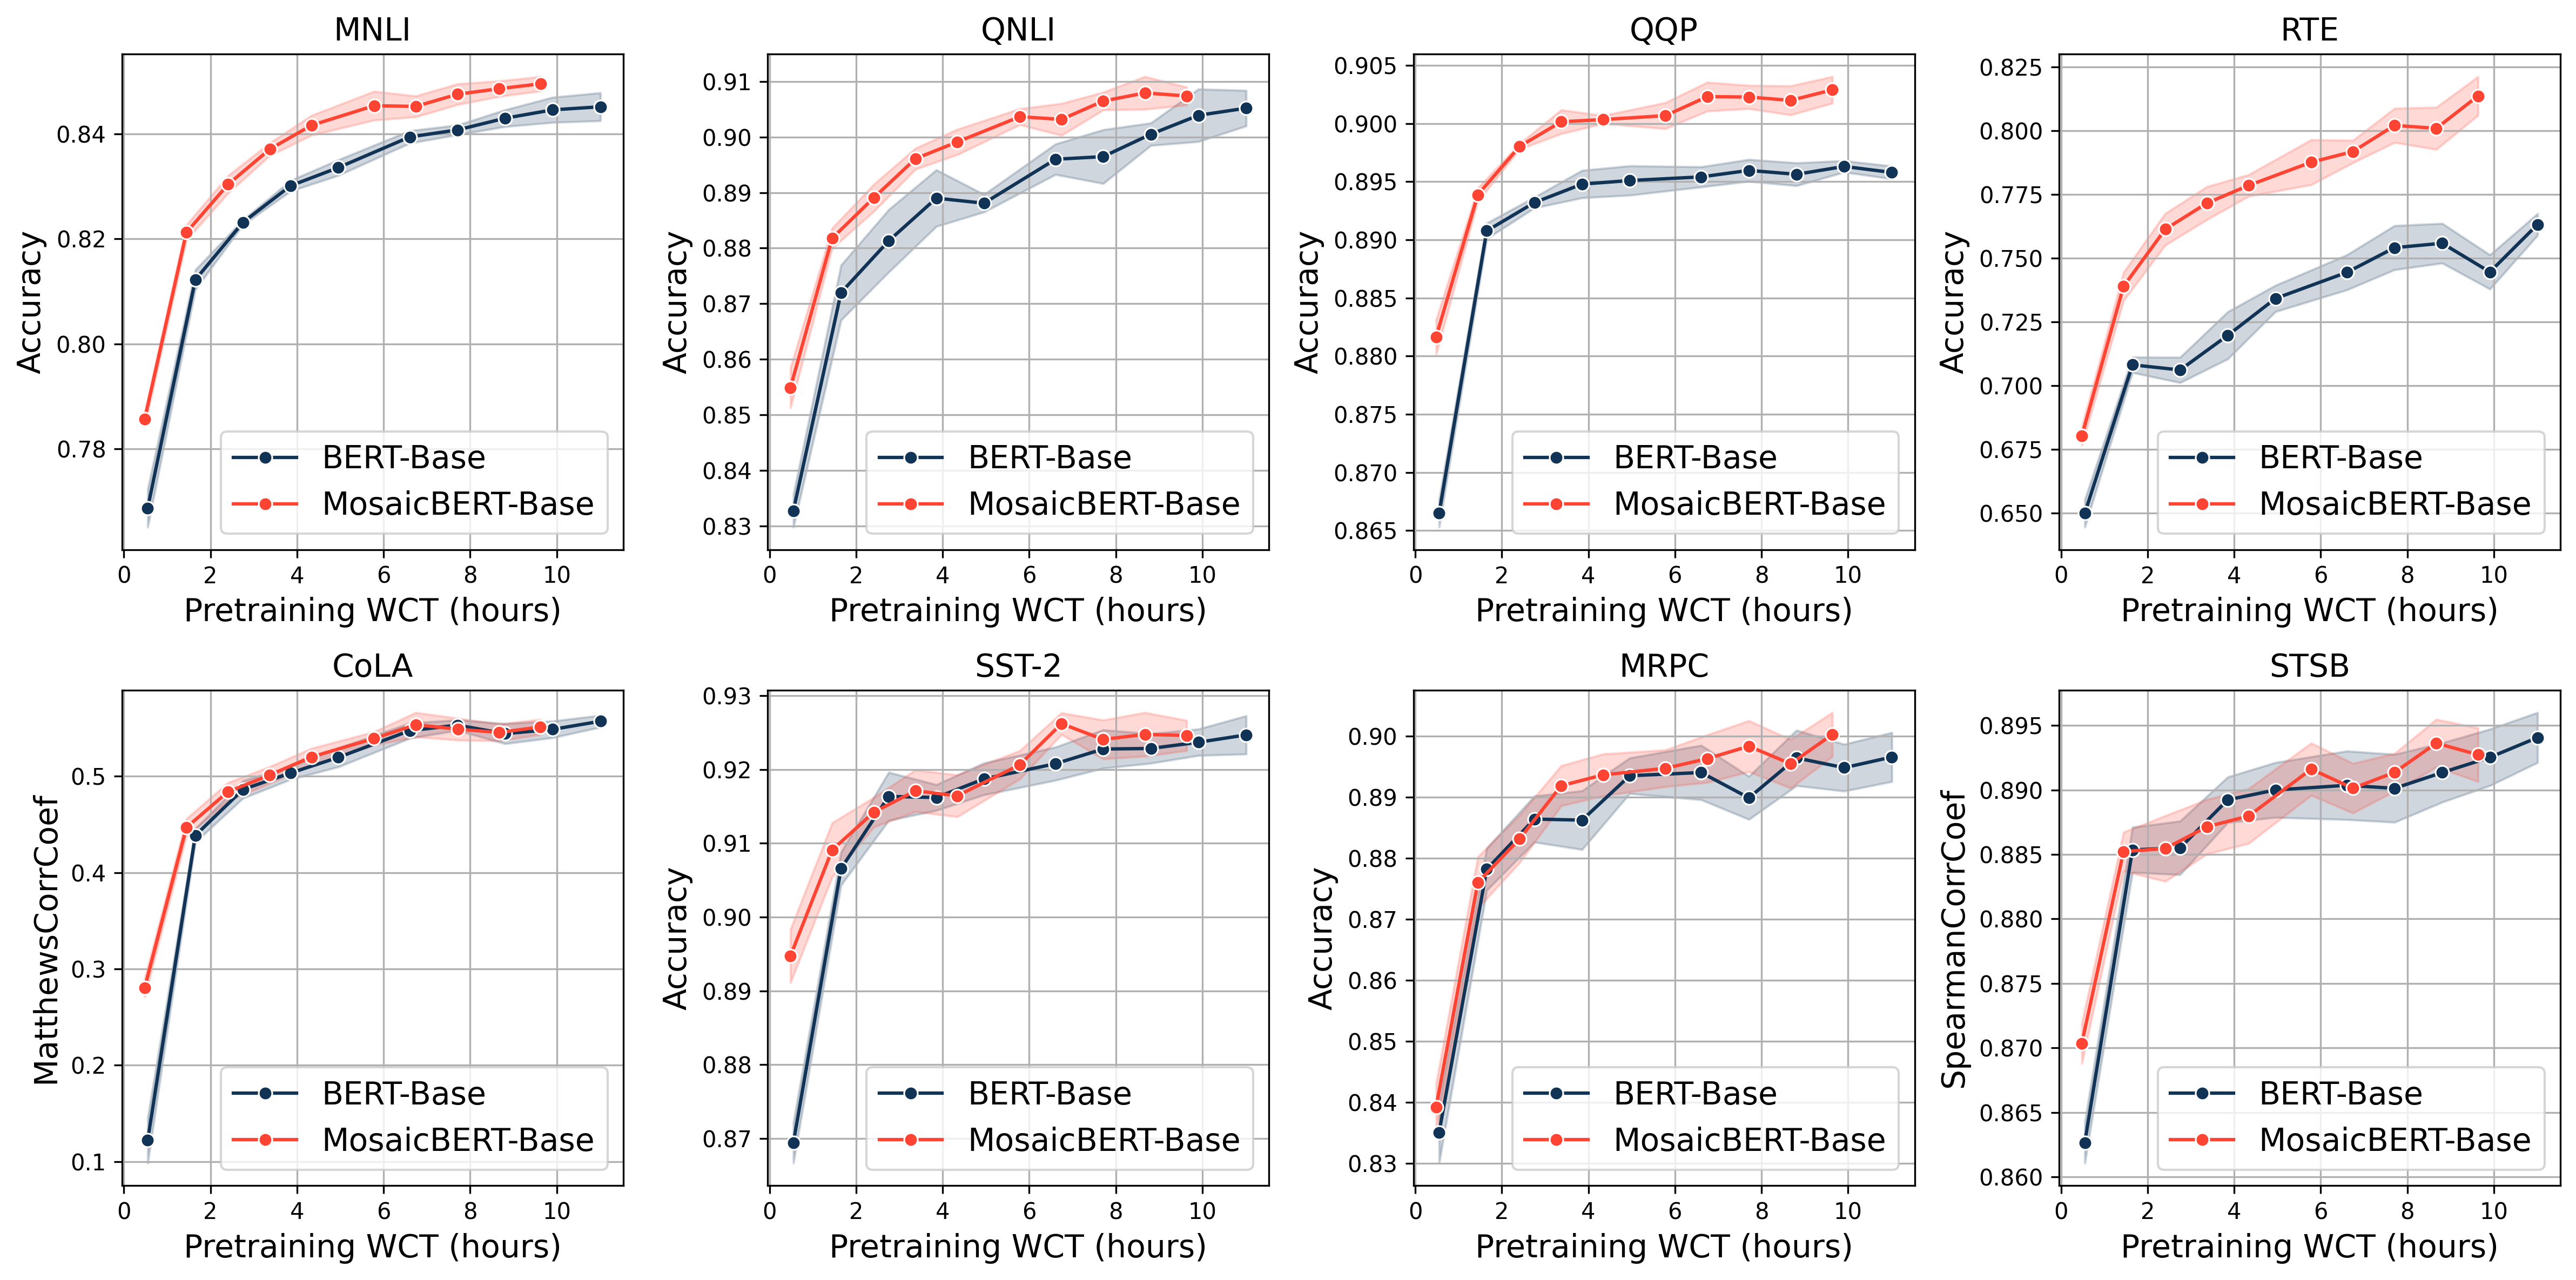
\includegraphics[width=\textwidth]{figures/bert-base-glue-individual-7-7-545pm.png}
    \caption{Performance on individual GLUE (dev) finetuning tasks. Our MosaicBERT-Base consistently outperforms BERT-Base on MNLI-m, QNLI, QQP and RTE, and has comparable performance on CoLA, SST-2, MRPC and STSB. Wall clock time is for $8\times$A100-80GB GPUs, and does not include finetuning time. Error bars are plotted with 95\% confidence interval across $n=5$ pretraining seeds, and all models are trained for 70,000 steps with batch size 4096.}
    \label{fig:bert_base_glue_individual}
\end{figure}



%%%%%%%%%%%
% RESULTS %
%%%%%%%%%%%

\section{Results}

In our first set of experiments, we pretrained BERT-Base and MosaicBERT-Base for 70,000 steps of batch size 4096, which roughly corresponds to 78\% of English C4 (Figure \ref{fig:intro_figure}B and Figure \ref{fig:bert_base_glue_individual}). We ran experiments with $n=5$ pretraining seeds for each model class. We then finetuned these models on the GLUE benchmark suite using identical finetuning parameters for all models and experiments; the details can be found in the Appendix.

\subsection{MosaicBERT-Base Achieves 79.6 Average GLUE (dev) Score in 1.13 Hours}

MosaicBERT-Base achieves the downstream average GLUE (dev) score of 79.6 in 1.13 hours on $8\times$A100 80 GB GPUs at a cost of roughly \$20 on a standard cloud provider. More details on cost estimates are included in the Appendix.

The baseline BERT-Base reached an average GLUE (dev) score of 83.2\% in 11.5 hours (A100-80GB), while MosaicBERT reached the same accuracy in roughly 4.6 hours on the same hardware, which is roughly a $2.38\times$ speedup (Table \ref{tab:bert_comparison} and Figure \ref{fig:intro_figure}B). 
%\todo{\textbf{TO DO: A few sentences describing costs and speed up (as per blog post). Missing info about AWS/GCP/Lambda costs for A100 40GB and 80GB}}

\subsection{MosaicBERT-Base is Pareto Optimal}

As can be seen Figure \ref{fig:intro_figure}B, MosaicBERT-Base consistently achieves higher average GLUE accuracy more quickly than the standard BERT-Base across all training durations. The performance of MosaicBERT on individual GLUE finetuning tasks can be seen in Figure \ref{fig:bert_base_glue_individual}. MosaicBERT-Base outperforms BERT-Base in four out of eight GLUE tasks across pretraining durations. 

The space of NLP benchmarks and tasks has exploded in recent years; we include more information on the individual tasks in the classic GLUE benchmark in the Appendix.
%\todo{should also explain somewhere why we chose to benchmark with GLUE}
MNLI, QNLI and QQP are the largest datasets in the GLUE benchmark, with 100k-400k training examples, and MosaicBERT-Base is strictly Pareto-optimal for these tasks relative to BERT-Base (Figure \ref{fig:bert_base_glue_individual}). We interpret this to mean that the architectural changes and training recipe we chose resulted in an optimized, efficient BERT-Base model.

The quality of both models on smaller datasets (3k-67k training samples) is much more variable, as shown by the large error bars (standard deviation across n=5 pretraining seeds) for SST-2, MRPC and STSB. Regardless of this variation, MosaicBERT-Base performs equivalently to BERT-Base on these tasks across training duration.


\begin{figure}
    \centering
    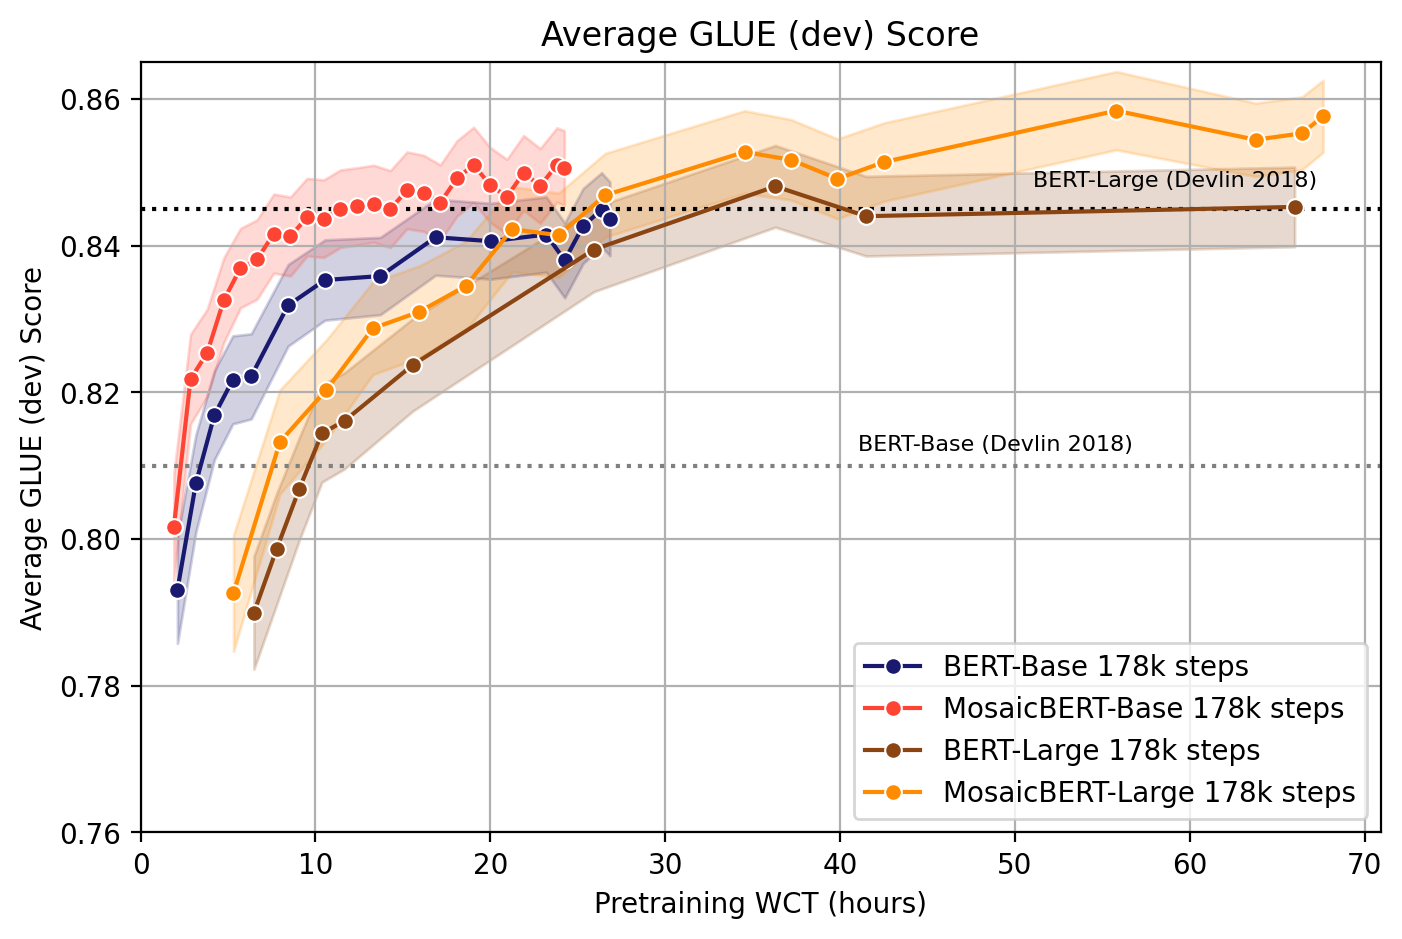
\includegraphics[width=0.8\textwidth]{figures/bert-large-av-glue-12-28-130pm.png}
    \caption{Average GLUE (dev) score Pareto curves for MosaicBERT-Base and Large trained for roughly 2 epochs of C4 (i.e. 178,000 steps with batch size 4096 with maximum sequence length 128 tokens). MosaicBERT-Base and Large are Pareto optimal relative to BERT-Base and Large. All pretraining is done on $8\times$A100 80GB devices (n=2-3 pretraining seeds). Note that BERT-Base and MosaicBERT-Base took much less time to train than BERT-Large and MosaicBERT-Large.}
    \label{fig:bert_large_glue_av}
\end{figure}

\subsection{MosaicBERT-Large is Pareto Optimal}

While BERT-Base is one of the most popular BERT models, BERT-Large comes in a close second. All of our model development was done on MosaicBERT-Base; we were therefore curious whether our architecture and pretraining choices also generalized to a larger model.

In a second set of experiments, we pretrained MosaicBERT-Base and Large as well as BERT-Base and Large for two epochs of the C4 dataset. The training duration is 178,000 steps with batch size 4096, and is more than twice as long as the duration of the models in Figures \ref{fig:intro_figure} and \ref{fig:bert_base_glue_individual}.

BERT-Large has 24 repeated transformer layers (BERT-Base has 12), and as a result consumes much more memory and takes longer to train. We found that MosaicBERT-Large reached an average GLUE score of 83.2 in 15.85 hours, while BERT-Large took 23.35 hours (Figure \ref{fig:bert_large_glue_av}).
%\todo{double check these numbers with new data} 
MosaicBERT-Large therefore had a $1.47\times$ speedup over BERT-Large in this training regime.

While MosaicBERT-Base is optimal for a constrained budget, the MosaicBERT-Large average GLUE score eventually surpasses MosaicBERT-Base after $25$ hours of training on a $8\times$A100-80GB node, and reaches an average score of 85.5 in roughly $50$ hours.
In our experiments, the MosaicBERT-Large architecture and pretraining was the same as MosaicBERT-Base, outside of the number of attention heads, number of hidden layers, and intermediate size of the feedforward units.

A striking result from Figures \ref{fig:bert_large_glue_av} and \ref{fig:bert_large_glue_individual} is that MosaicBERT-Base is Pareto optimal relative to BERT-large in this training regime, and is Pareto optimal to MosaicBERT-Large during the first half of training.  MosaicBERT-Base takes only $25$ hours to complete 2 epochs, while MosaicBERT-Large takes close to $70$ to complete 2 epochs. A potential takeaway from this is that MosaicBERT-Large only surpasses Base performance in the large data regime. For certain tasks such as QQP, SST-2, and MRPC MosaicBERT-Base achieves a maximum accuracy on par with the maximum accuracy of MosaicBERT-Large, for far fewer pretraining hours. When building encoders for specific domains and tasks, bigger is not always better.



% \begin{figure}
%     \centering
%     \includegraphics[width=1\textwidth]{figures/bert-large-individual-glue-7-7-723pm.png}
%     \caption{MosaicBERT-Base and Large accuracy (dev) vs. pretraining speed Pareto curves for individual GLUE benchmarks. All models were trained on 2 epochs of C4 (178,000 steps with batch size 4096). Error bars represent 95\% confidence interval for n=2-3 pretraining seeds. Dashed black line represents BERT-Large accuracy on the GLUE (dev) data \citep{devlin2018bert,liu2019roberta}.}
%     \label{fig:bert_large_glue_individual}
% \end{figure}


\begin{figure}
    \centering
    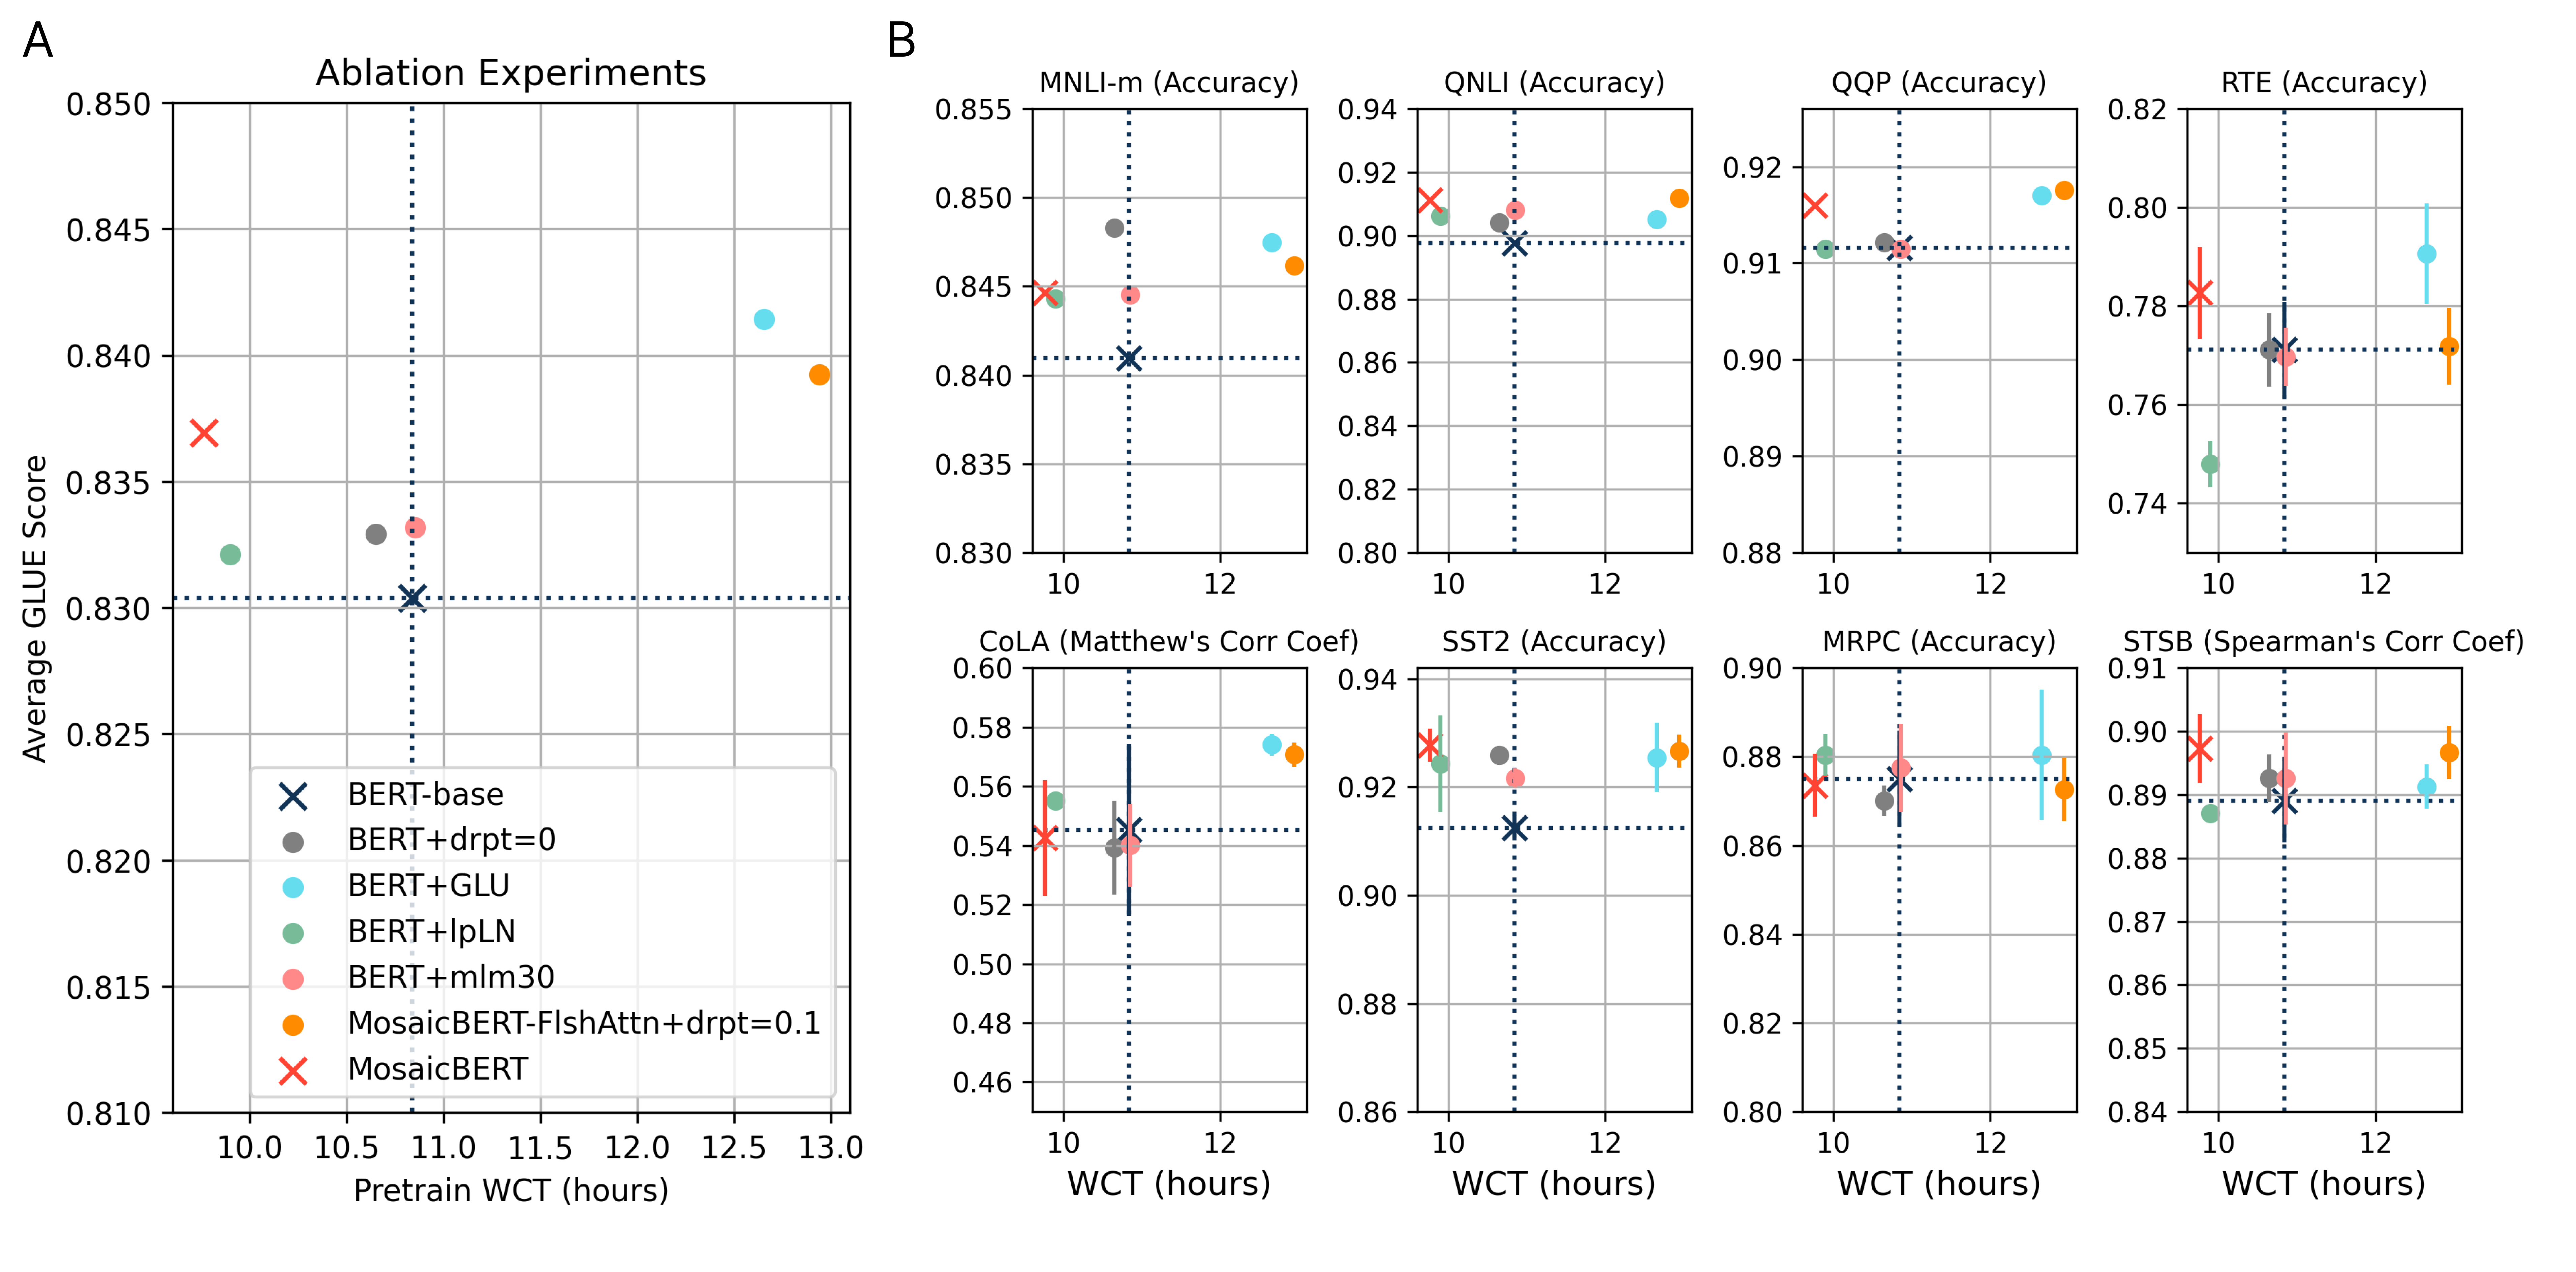
\includegraphics[width=1\textwidth]{figures/ablation-experiments-v2.png}
    \caption{Ablation Experiments (A) Average GLUE score and (B) Individual GLUE tasks. \textbf{BERT-base}: standard BERT-base (110M parameters) with attention dropout=0.1 and feedforward dropout=0.1, vocab size set to 30522, MLM=15\% (all Hugging Face standard configurations). \textbf{BERT+drpt=0}: standard BERT-base, except that the attention in the dropout layer is set to 0 instead of the default 0.1. \textbf{BERT+GLU}: standard BERT-base, with GLU for the feedforward component of the encoder block. \textbf{BERT+lpLN}: standard BERT-base, except with low precision LayerNorm (bfloat16). \textbf{BERT+mlm30}: standard BERT-base, except with a masked language modeling masking ratio of 30\%. \textbf{MosaicBERT}: the complete MosaicBERT-Base including GLU (where the dimension of the intermediate layer is 3072 resulting in 137M total parameters), ALiBi, low precision LayerNorm, unpadding, MLM 30\%, vocab size 30528 (a multiple of 64) and the attention dropout=0. \textbf{MosaicBERT-FlashAttn+drpt=0.1}: MosaicBERT-Base \textit{without} Flash Attention and \textit{with} the attention dropout set to 0.1.}
    \label{fig:ablation_experiments}
\end{figure}

\subsection{Ablation Experiments}

When deciding on the final setup for MosaicBERT, we tried to make educated guesses about what combination of modifications could work well together to both increase FLOP utilization and maintain or improve accuracy. Our approach was inspired by Amdahl's Law, i.e. the idea that optimizing a portion of a system responsible for N\% of the costs can lead to, at most, an N\% speedup \citep{rodgers1985improvements}, and chose each of the modifications such that they did not target the same exact part of the of the stack. For example, low precision LayerNorm and GLU affect different parts of the encoder block, and so potentially compose well.

In the following ablation experiments we benchmark the individual effects of various architecture and training choices on pretraining wall clock time. We plot downstream GLUE accuracy as a function of measured pretraining wall clock time in Figure \ref{fig:ablation_experiments}. 

The patterns in Figure \ref{fig:ablation_experiments}A-B shed light on the individual effects of various architectures (e.g. BERT+GLU, BERT+low precision LayerNorm) and training configurations (e.g. BERT + 30\% masking ratio). On average, all methods seem to provide a slight accuracy boost to BERT-base. Increasing the masking ratio to 30\% leads to a slight accuracy boost while not affecting the WCT, while turning off dropout in the attention layer (BERT+drpt=0) leads to a slight improvement in both accuracy and WCT. Low precision LayerNorm (BERT+lpLN) leads to a significant speedup (i.e. a shift to the left). Gated Linear Units (BERT+GLU) add more parameters to the model and lead to a significant slowdown while providing an accuracy boost. As a point of reference, we also benchmark the full MosaicBERT as well as MosaicBERT without FlashAttention and with attention dropout set to 0.1 (the standard BERT-base configuration).




In these experiments, all BERT-Base models here were pretrained on C4 for 70,000 steps with batch size 4096, and microbatch size 256 on 8$\times$A100 80GB GPUs. All models were initialized with the same seed and shared all other hyperparameters including the bert-base uncased tokenizer, the learning rate schedule, AdamW as the optimizer, etc. Final pretraining checkpoints were then finetuned on GLUE following the details in the appendix. The points represented in these GLUE plots are final finetuning checkpoints.

These plots highlight the importance of benchmarking with Pareto curves, as it is not possible to tell from these plots alone whether training BERT-base for 2 more hours leads to better performance than BERT+GLU, for example.


%%%% This section describes Alex's experiments from July 2022 combining Fused LayerNorm, ALiBi and GLU
%%% This text was used for the original submission
% How do each of the architecture modifications affect throughput during training? We ran a series of experiments looking at the individual and combinatorial effects of low precision LayerNorm, ALiBi and GLU on the baseline BERT-Base. 
% As can be seen from Figure \ref{fig:throughput_barplot}A, ALiBi has a marginal effect on the throughput as measured by samples per second, while GLU leads to a decrease in throughput. Low precision LayerNorm alone causes an \textit{increase} in throughput, due to the reduced floating point precision.
% When low precision LayerNorm, ALiBi and GLU are combined together on top of the baseline BERT, the throughput gains of low precision LayerNorm are cancelled out by the slowdown due to GLU.

% In Figure \ref{fig:throughput_barplot}B, we show the throughput of the ``complete'' MosaicBERT-Base with differently-sized GLU matrices of intermediate size 2048 and 3072. While MosaicBERT-Base with GLU-2048 has the highest throughput, we found that the added expressivity of GLU-3072 due to the increase in parameters compensated for the relative decrease in throughput, and therefore used this configuration for the modeling in Figures \ref{fig:intro_figure}-\ref{fig:bert_large_glue_individual}.

% Since \citet{dao2022flashattention} showed that FlashAttention leads to an increase in throughput without any decrease in accuracy, and \citet{zeng2022boosting} showed that removing padding leads to an increase in throughput, we do not include those ablation experiments here.

% \subsection{Result 5 - Extrapolation to Long Sequences with ALiBi}\todo{I would like to put this in the Appendix giving the current timing}
% ALiBi allows for extrapolation
% Can train on 128 and finetune on 256/512 etc. How do we show this??!!
% \begin{itemize}
%     \item “Train short test long” (ie zero shot)
%     \item “Train on short and finetune long”
% \end{itemize}

% This could be difficult to show if we don’t compare to a baseline model that is also finetuned on long sequences. Note flash attention is linear in memory, quadratic in time

% Question - are RoBERTa and DeBERTa also sinusoidal positional encoding? How about the encoder from T5?

% Is zero shot the only benefit of ALiBi?


\section{Related Work}

Various studies rightly focus on a single method or modification that improves throughput, such as FlashAttention \cite{dao2022flashattention} and unpadding \citep{zeng2022boosting}. In this study, we incorporate many of these techniques to investigate whether they combine advantageously.

RoBERTa (``Robustly optimized BERT approach'') is the most influential work in this regard \citep{liu2019roberta}. In this study, they kept the exact BERT architecture but changed the training recipe by removing the next sentence prediction objective, training for longer on much larger datasets, and changing the batch size, among other things. They showed that the original BERT was significantly undertrained - while the original BERT trained on 16GB worth of text, the top accuracy RoBERTa (Large) was trained on 160GB of data for 500,000 steps with batch size 8192. Many of the training choices in RoBERTa have become standard practice; our training recipe therefore more closely resembles RoBERTa than the original BERT. See Appendix for a more detailed comparison of RoBERTa and MosaicBERT.

%they showed that the original BERT was significantly undertrained and di
%\textbf{TO DO}RoBERTa (Robustly optimized BERT approach)- showed that BERT was significantly undertrained.  Did not change the architecture itself. Used sequence length 512. Use five English-language corpora  160GB of text. They did\textit{not} make any architectural changes\footnote{They note that ``Studying architectural changes, including larger architectures, is an important area for future work.''}.  Also use a larger vocabulary (50k) instead of 30k. This adds additional parameters to the model.  



Improvements in transformer architecture and GPU hardware have caused the cost of pretraining BERT models to decline precipitously.
The recent paper “Cramming: Training a Language Model on a Single GPU in One Day” \citep{geiping2023cramming} exemplifies this trend. The goal of this rigorous study was to train the best BERT in 24 hours on a single GPU. Similar to us, they tweaked the BERT architecture to incorporate FlashAttention and Gated Linear Units (but without increasing the dimensionality of the hidden block). Unlike MosaicBERT, they used scaled sinusoidal positional embeddings \citep{vaswani2017attention} as well as Pre-LayerNorm (applying LayerNorm before the attention and feedforward layers) and did not change the pretraining masking rate. With this setup, they were able to train their modified BERT-Base to an average GLUE score of 80.4 in 24 hours on a single A6000 GPU (i.e. 24 GPU hours, as per Table 3 of \citep{geiping2023cramming}). Our study is similar in spirit, but asks what is the fastest architecture for pretraining, and expands on this in greater detail by showing that MosaicBERT is Pareto optimal relative to BERT.

% Geiping played with C4 just a bit

While we believe that our training optimization choices for MosaicBERT go a long way to improve BERT training efficiency, there are likely further modifications that could lead to an increase in accuracy with no effect on throughput, such as replacing LayerNorm with RMSNorm \citep{zhang2019root} and GeGLU with SwiGLU \citep{shazeer2020glu,narang2021transformer}. Removing all biases from the linear layers can also potentially lead to slight speed ups in training time without a significant hit to accuracy. ``NarrowBERT'' \citep{li2023narrowbert} suggested a clever change to the way encoder blocks are stacked so that computation is not wasted on unmasked tokens. Another recent study showed that dynamically masking the masking ratio during pretraining leads to downstream accuracy gains in BERT \cite{ankner2023dynamic}.  Note, however, that accounts such as \citep{geiping2023cramming} and \citep{kaddour2023no} document many examples where certain modifications to the BERT architecture and training recipe fail to improve accuracy. We also note here that there is an ongoing debate about the benefits of RoPE (rotary positional embeddings) \citep{su2024roformer} versus AliBi \citep{press2021train}. Finally, using a more modern tokenizer will likely have an effect on downstream accuracy \citep{geiping2023cramming}.

Approaches such as knowledge distillation \citep{blakeney2022reduce} might additionally push the Pareto frontier of BERT models during pretraining and finetuning. Progressive layer stacking is one example technique; by initializing a larger BERT model with the weights from smaller pretrained BERT models, pretraining can be reliably accelerated \citep{gong2019efficient,kaddour2023no}. As the field is learning how to optimize stable model training at the billion parameter scale \citep{chowdhery2022palm,dehghani2023scaling}, we expect some of these innovations to cycle back to smaller models such as BERT-Base. For example, it has been hypothesized that incorporating more LayerNorm modules at the QK matrix output (i.e. QK-LayerNorm \citep{henry2020query}) can lead to improved stability during training; combining this with a more aggressive learning rate schedule could lead to faster convergence.

\section{Discussion}
**How does MosaicBERT optimize for fast pretraining compared to traditional BERT models?**

MosaicBERT optimizes for fast pretraining compared to traditional BERT models through a combination of architectural modifications and training recipe improvements. These optimizations include incorporating FlashAttention, ALiBi, GLU, dynamic unpadding module, and low precision LayerNorm in the encoder architecture [4]. Additionally, MosaicBERT uses a 30\% masking ratio for Masked Language Modeling (MLM) objective, bfloat16 precision, and vocabulary size optimized for GPU throughput [1]. By implementing these changes, MosaicBERT achieves a high GLUE score in a significantly shorter pretraining time of 1.13 hours on 8 GPUs at a lower cost compared to traditional BERT models [1]. The study demonstrates the Pareto optimality of MosaicBERT in terms of pretraining speed and accuracy through extensive accuracy vs. training time Pareto curve comparisons [2]. Furthermore, MosaicBERT offers researchers and engineers an efficient way to pretrain custom BERT-style models at a faster speed and lower cost, thus opening up opportunities for advancements in natural language processing research [1].

**Can you provide more details on how MosaicBERT incorporates FlashAttention, ALiBi, GLU, dynamic unpadding module, and low precision LayerNorm in its encoder architecture to optimize for fast pretraining?**

MosaicBERT incorporates several architectural choices to optimize for fast pretraining.

First, it utilizes FlashAttention, which reduces the number of read/write operations between GPU memory, improving efficiency [4a]. This is combined with Attention with Linear Biases (ALiBi), which eliminates position embeddings and encodes position information directly through the attention operation, biasing attention to nearby tokens and allowing for extrapolation to longer context lengths [4b].

Additionally, MosaicBERT includes Gated Linear Units (GLU) and a dynamic unpadding module. GLU enhances the nonlinear interactions between different tokens, while the dynamic unpadding module removes padded tokens during training, reducing wasted operations on padding tokens [5a][5b].

Finally, MosaicBERT utilizes low precision LayerNorm, running the LayerNorm modules in bfloat16 precision instead of float32 to reduce memory requirements without experiencing numerical instabilities [5c].

By incorporating these modifications into its encoder architecture, MosaicBERT is optimized for fast pretraining, achieving high efficiency and performance in natural language processing tasks at a lower cost and faster speed.

**Can you explain more about the function of the dynamic unpadding module in MosaicBERT?**

The dynamic unpadding module in MosaicBERT is a modification that changes the standard practice of padding sequences of different lengths with special padding tokens in natural language processing tasks. Instead of padding each sequence individually, the dynamic unpadding module concatenates all examples from a minibatch into a single sequence of batch size 1. This approach eliminates the need to perform operations on padding tokens during training, leading to speed improvements. Research by NVIDIA and others has shown that this method can enhance training efficiency by reducing the wasted operations on padding tokens [66]. In summary, the dynamic unpadding module in MosaicBERT optimizes training speed by streamlining the processing of text sequences during pretraining tasks in NLP research.

**Are there any potential drawbacks to using the dynamic unpadding module in MosaicBERT, such as increased memory usage or longer training times?**

The dynamic unpadding module in MosaicBERT does not appear to have any potential drawbacks in terms of increased memory usage or longer training times. In fact, the module is implemented to improve training efficiency by removing operations on padding tokens, leading to speed improvements during training [5]. Overall, the modifications introduced in MosaicBERT, including the dynamic unpadding module, are aimed at optimizing pretraining efficiency without sacrificing accuracy or increasing resource requirements [1]. Therefore, it can be inferred that the dynamic unpadding module in MosaicBERT is designed to enhance training speed rather than introduce any negative effects on memory usage or training duration.

**Can you explain the concept of Pareto optimality as demonstrated in the study, and how it relates to the trade-offs between pretraining speed and accuracy?**

Pareto optimality, as demonstrated in the study, refers to finding the best possible trade-off between two conflicting objectives, in this case, pretraining speed and accuracy. By plotting accuracy vs. training time Pareto curves, the study shows that MosaicBERT is Pareto optimal relative to traditional BERT models across different training durations. This means that MosaicBERT achieves superior accuracy within various training budgets while keeping other factors constant[16].

The study uses Pareto curves to compare different models and configurations based on how they balance accuracy and training time. These curves help assess the trade-offs between architectural changes that may improve efficiency but have different effects on speed and accuracy. By generating and analyzing Pareto curves, the study provides a comprehensive view of how different choices in model architecture and training impact the overall performance[2].

In essence, Pareto optimality in this study highlights how architectural modifications in MosaicBERT lead to improvements in both pretraining speed and accuracy compared to traditional BERT models, showcasing the benefits of optimizing the model for efficiency in natural language processing research.

\section{Conclusion} 

In this study we show how combinations of architecture choices can improve BERT pretraining speed and accuracy.
We built MosaicBERT to enable ML researchers and engineers to pretrain BERT models from scratch on their own data and build better models for their specific domains without facing time and cost restrictions. We ultimately hope that by making BERT training faster and cheaper, our work contributes to the trend in NLP research away from finetuning generic models and towards of pretraining custom encoders on domain specific data.
A large body of research has highlighted the success of BERT-style models pretrained on a specific domains  such as biomedicine \citep{beltagy2019scibert,lee2020biobert,gu2021domain,el2022re}, math \citep{shen2021mathbert}, chemistry \citep{bai2021pre,horawalavithana2022foundation}, financial communications \citep{shah2022flue}, and code \citep{tabassum2020code}. This seems to hold true even in the age of LLMs \citep{bioMedLM,wu2023bloomberggpt}.

\subsection*{Code}
A stable webpage for this work can be found at \href{https://mosaicbert.github.io}{\url{mosaicbert.github.io}}. Code for pretraining and finetuning MosaicBERT can be found in the MosaicML \url{examples} repository \href{https://github.com/mosaicml/examples}{\url{https://github.com/mosaicml/examples}}. The exact code for this study was pinned to \url{v0.0.4} of the MosaicML \url{mosaicml/examples} repository \href{https://github.com/mosaicml/examples/tree/v0.0.4/examples/bert}{\url{https://github.com/mosaicml/examples/tree/v0.0.4/examples/bert}}. 
All pretraining and finetuning was done in PyTorch 1.13 using the MosaicML \texttt{Composer} library \href{https://github.com/mosaicml/composer}{\url{https://github.com/mosaicml/composer}}. 
Model weights for MosaicBERT-Base can be found on the HuggingFace hub \href{https://huggingface.co/mosaicml/mosaic-bert-base}{\url{https://huggingface.co/mosaicml/mosaic-bert-base}}.

Code for pretraining and finetuning transformers such as MPT and derivative versions of MosaicBERT can be found in the MosaicML \url{llm-foundry} repository \href{https://github.com/mosaicml/llm-foundry}{\url{https://github.com/mosaicml/llm-foundry}}.

\subsection*{Acknowledgements}
The authors would like to thank Erica Yuen, Vitaliy Chiley, Connor Jennings, and Aaron Gokaslan for their feedback on the code and manuscript. We would also like to thank Ishana Shastri and Vlad Ivanchuk for some of their early work as interns that led to MosaicBERT. The majority of this work appeared as a blogpost with the title \href{https://www.mosaicml.com/blog/mosaicbert}{``MosaicBERT: Pretraining BERT from Scratch for \$20''} in March 2023.\footnote{\href{https://www.mosaicml.com/blog/mosaicbert}{\url{mosaicml.com/blog/mosaicbert}}} This work also builds on the MosaicML MLPerf v2.1 results for BERT-Large \citep{mosaicml2022mlperf}.









% \begin{figure}[h!]
%     \centering
%     \includegraphics[width=0.8\textwidth]{figures/example-image.png}
%     \caption{EXAMPLE FIGURE - THROUGHPUT COMPARISON OF DIFFERENT METHODS}
%     \label{fig:my_label}
% \end{figure}

\newpage

\bibliography{sources}
\bibliographystyle{abbrvnat}

%%%%%%%%%%%%%%%%%%%%%%%%%%%%%%%%%%%%%%%%%%%%%%%%%%%%%%%%%%%%

\newpage

\appendix
\beginsupplement

\subfile{appendix.tex}

\end{document}